% Three-drone scenario: cable 0 snaps at t=7.0s
% Three panels: pre-fault (t=6.0), transient (t=7.5), settled (t=12.0)
% Shows XY-plane relative positions (drone - load) to highlight formation geometry
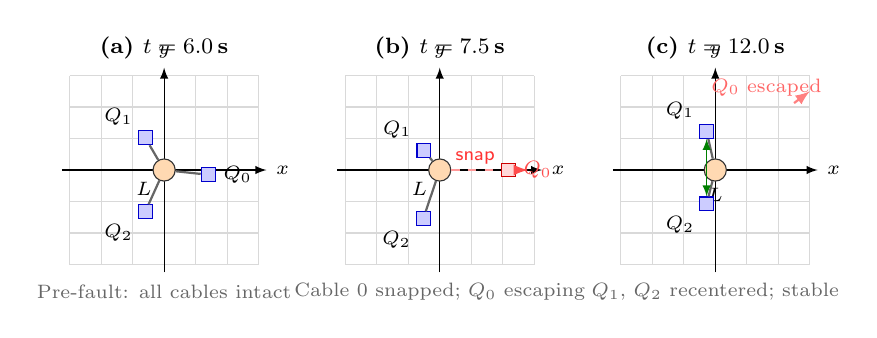
\begin{tikzpicture}[
  drone/.style={draw=blue!80!black, fill=blue!20, minimum size=5pt, inner sep=0pt, font=\tiny},
  faulted/.style={draw=red!80!black, fill=red!15, minimum size=5pt, inner sep=0pt, font=\tiny},
  escaped/.style={draw=red!60, fill=red!5, minimum size=5pt, inner sep=0pt, dashed, font=\tiny},
  payload/.style={circle, draw=black!80, fill=orange!30, minimum size=8pt, inner sep=0pt},
  cable/.style={thick, black!60},
  snapped/.style={thick, red!40, dashed},
  panel/.style={font=\footnotesize\bfseries},
  lbl/.style={font=\scriptsize},
  >=latex
]

% === Panel (a): t = 6.0 s — Pre-fault ===
\begin{scope}[shift={(0,0)}]
  \draw[gray!30, thin] (-1.2,-1.2) grid[step=0.4] (1.2,1.2);
  \draw[->] (-1.3,0) -- (1.3,0) node[right, font=\scriptsize]{$x$};
  \draw[->] (0,-1.3) -- (0,1.3) node[above, font=\scriptsize]{$y$};

  % Payload at origin (relative coords)
  \node[payload] (L) at (0,0) {};
  \node[lbl, below left=1pt] at (L) {$L$};

  % Drone positions relative to load at t=6.0
  \node[drone] (D0) at (0.56, -0.06) {};
  \node[drone] (D1) at (-0.24, 0.41) {};
  \node[drone] (D2) at (-0.24, -0.53) {};

  % Cables
  \draw[cable] (L) -- (D0);
  \draw[cable] (L) -- (D1);
  \draw[cable] (L) -- (D2);

  % Labels
  \node[lbl, right=2pt] at (D0) {$Q_0$};
  \node[lbl, above left=1pt] at (D1) {$Q_1$};
  \node[lbl, below left=1pt] at (D2) {$Q_2$};

  \node[panel] at (0, 1.55) {(a) $t = 6.0$\,s};
  \node[lbl, text=black!60] at (0, -1.55) {Pre-fault: all cables intact};
\end{scope}

% === Panel (b): t = 7.5 s — 0.5 s after snap ===
\begin{scope}[shift={(3.5,0)}]
  \draw[gray!30, thin] (-1.2,-1.2) grid[step=0.4] (1.2,1.2);
  \draw[->] (-1.3,0) -- (1.3,0) node[right, font=\scriptsize]{$x$};
  \draw[->] (0,-1.3) -- (0,1.3) node[above, font=\scriptsize]{$y$};

  % Payload at origin
  \node[payload] (L) at (0,0) {};
  \node[lbl, below left=1pt] at (L) {$L$};

  % Drone positions relative to load at t=7.5
  \node[faulted] (D0) at (0.87, 0.00) {};
  \node[drone] (D1) at (-0.20, 0.25) {};
  \node[drone] (D2) at (-0.21, -0.62) {};

  % Cables: cable 0 snapped
  \draw[snapped] (L) -- (D0);
  \draw[cable] (L) -- (D1);
  \draw[cable] (L) -- (D2);

  % Escape arrow
  \draw[->, red!70, thick] (D0) -- ++(0.25, 0.0);

  % Snap marker
  \node[font=\scriptsize, red!80] at (0.45, 0.15) {\textsf{snap}};

  % Labels
  \node[lbl, right=2pt, red!70] at (D0) {$Q_0$};
  \node[lbl, above left=1pt] at (D1) {$Q_1$};
  \node[lbl, below left=1pt] at (D2) {$Q_2$};

  \node[panel] at (0, 1.55) {(b) $t = 7.5$\,s};
  \node[lbl, text=black!60] at (0, -1.55) {Cable 0 snapped; $Q_0$ escaping};
\end{scope}

% === Panel (c): t = 12.0 s — Settled ===
\begin{scope}[shift={(7.0,0)}]
  \draw[gray!30, thin] (-1.2,-1.2) grid[step=0.4] (1.2,1.2);
  \draw[->] (-1.3,0) -- (1.3,0) node[right, font=\scriptsize]{$x$};
  \draw[->] (0,-1.3) -- (0,1.3) node[above, font=\scriptsize]{$y$};

  % Payload at origin
  \node[payload] (L) at (0,0) {};
  \node[lbl, below=3pt] at (L) {$L$};

  % Drone positions relative to load at t=12.0
  % D0 is at (5.92, 4.15) relative -- far off-screen
  \node[drone] (D1) at (-0.11, 0.49) {};
  \node[drone] (D2) at (-0.11, -0.43) {};

  % Cables
  \draw[cable] (L) -- (D1);
  \draw[cable] (L) -- (D2);

  % Off-screen arrow for D0
  \draw[->, red!50, thick, dashed] (1.0, 0.85) -- (1.2, 1.0);
  \node[lbl, red!60] at (0.65, 1.05) {$Q_0$ escaped};

  % Labels
  \node[lbl, above left=1pt] at (D1) {$Q_1$};
  \node[lbl, below left=1pt] at (D2) {$Q_2$};

  % Recentered annotation
  \draw[<->, green!50!black, thin] (D1) -- (D2);

  \node[panel] at (0, 1.55) {(c) $t = 12.0$\,s};
  \node[lbl, text=black!60] at (0, -1.55) {$Q_1$, $Q_2$ recentered; stable};
\end{scope}

\end{tikzpicture}
